% This is the Reed College LaTeX thesis template. Most of the work 
% for the document class was done by Sam Noble (SN), as well as this
% template. Later comments etc. by Ben Salzberg (BTS). Additional
% restructuring and APA support by Jess Youngberg (JY).
% Your comments and suggestions are more than welcome; please email
% them to cus@reed.edu
%
% See http://web.reed.edu/cis/help/latex.html for help. There are a 
% great bunch of help pages there, with notes on
% getting started, bibtex, etc. Go there and read it if you're not
% already familiar with LaTeX.
%
% Any line that starts with a percent symbol is a comment. 
% They won't show up in the document, and are useful for notes 
% to yourself and explaining commands. 
% Commenting also removes a line from the document; 
% very handy for troubleshooting problems. -BTS

% As far as I know, this follows the requirements laid out in 
% the 2002-2003 Senior Handbook. Ask a librarian to check the 
% document before binding. -SN

%%
%% Preamble
%%
% \documentclass{<something>} must begin each LaTeX document
\providecommand{\main}{..}
\documentclass[12pt,twoside,class=../reedthesis, crop=false]{standalone}
% Packages are extensions to the basic LaTeX functions. Whatever you
% want to typeset, there is probably a package out there for it.
% Chemistry (chemtex), screenplays, you name it.
% Check out CTAN to see: http://www.ctan.org/
%%
\usepackage{graphicx,latexsym} 
\usepackage{amssymb,amsthm,amsmath}
\usepackage{longtable,booktabs,setspace} 
\usepackage{chemarr} %% Useful for one reaction arrow, useless if you're not a chem major
\usepackage[hyphens]{url}
\usepackage{rotating}
\usepackage{hyperref}

\usepackage{physics}
\usepackage{siunitx}
\usepackage{xcolor}
% \usepackage{standalone}
% \usepackage{natbib}
% Comment out the natbib line above and uncomment the following two lines to use the new 
% biblatex-chicago style, for Chicago A. Also make some changes at the end where the 
% bibliography is included. 
%\usepackage{biblatex-chicago}
%\bibliography{thesis}

% \usepackage{times} % other fonts are available like times, bookman, charter, palatino

\providecommand{\zcut}{\mathrm{z_{cut}}}


\setlength{\parskip}{0pt}
%%
%% End Preamble
%%
%% The fun begins:
\begin{document}
	The first step on the path to an all-orders calculation is to derive a factorization formula for the heavy hemisphere mass cross section. The basic process for doing so is laid out in technical detail in Ref.~\cite{becher_introduction_2015-1}, and an example of a similar flavor to our calculation is provided by Frye et al.\ in Ref.~\cite{frye_factorization_2016}.\footnote{Indeed, the calculation of Frye et al.\ is a more general factorization of mass-like variables in groomed jets. Setting $\alpha = 2, \beta = 0$ for their two-point energy correlation function $e_2^{(\alpha)}$ under soft drop grooming with angular exponent $\beta$ yields the mMDT-groomed jet mass $\rho$. Their factorization is valid in the limit $\rho \ll \zcut \ll 1$, whereas we are interested in the limit $\rho \sim \zcut \ll 1$.} There are two primary steps in developing a factorization formula:
	\begin{enumerate}
		\item \textbf{Power counting}: this involves determining the possible radiative modes of an event and their dominant momentum scales. The term `power counting' refers to the fact that for some momentum scale $\lambda$, different radiative modes have momenta that scale as different powers of $\lambda$.

		\item \textbf{Factorization and refactorization}: Once the different radiative modes and energy scales are identified, we can use the framework of SCET to split the cross section into a convolution of terms describing different radiative modes. These terms themselves must then be split (refactored) into convolutions of terms, each of which depends, to leading order, only on a single energy scale.
	\end{enumerate}

\section{Setup}
	Recall that the hemisphere mass is defined to be
	\begin{equation}
		\rho = \frac{1}{E_J^2} \sum_{i<j} 2p_i \cdot p_j
	\end{equation}
	with $E_J$ the jet energy and the sum ranging over all pairs of particles in the jet. Expanding out the dot product, we have
	\begin{equation}\label{eq:jet mass z theta}
		\rho = \frac{2}{E_J^2} \sum_{i<j} \qty(E_i E_j - \vb{p}_i \cdot \vb{p}_j) = \frac{2}{E_J^2} \sum_{i<j} E_i E_j \qty(1 - \cos\theta_{ij}) = \sum_{i<j}2z_i z_j \qty(1 - \cos\theta_{ij}).
	\end{equation}
	Here, $z_i$ and $z_j$ are the relative energy fractions of each particle and $\theta_{ij}$ is the angle between particles $i$ and $j$.

	Throughout the following discussion, with $n^\mu$ the jet direction and $\bar n^\mu$ the direction opposite the jet, we will describe momenta in light-cone coordinates
	\begin{equation}
		p^\mu = \qty(p^-, p^+, p_\perp)
	\end{equation}
	with
	\begin{align}
		p^- &= \bar n \cdot p & p^+ &= n \cdot p
	\end{align}
	and $p_\perp$ the components of momentum transverse to $n$. In these coordinates, the energy fraction with respect to total energy $E_J = Q$ is
	\begin{equation}\label{eq:z light cone coordinates}
		z = \frac{p^+ + p^-}{2Q}
	\end{equation}
	and, in the collinear limit, the angle to the jet axis is $\theta \approx p_\perp / p^0$ \cite{frye_factorization_2016}.
	
	In an $e^+ e^- \to \text{jets}$ event, there are two types of emission: resolved and unresolved. The essential difference is that a resolved emission is one which manifests itself as a jet at a particular scale of observation, while an unresolved emission does not. The presence of unresolved emissions can, however, perturb observable values of a resolved emission. {\color{red}\textbf{[TODO: check that this is a reasonable description]}} 

	Suppose now that we have applied an mMDT groomer with energy fraction cutoff $\zcut$. Then every \textit{resolved} emission must satisfy
	\begin{equation}
		z_i > \zcut,
	\end{equation}
	while other emissions with $z_i < \zcut$ can only pass the groomer if they are at a sufficiently small angle to a resolved emission.

\section{Power counting}
\subsection{Resolved soft emission}
	The primary emission contributing to the jet mass in the limit $\rho \sim \zcut \ll 1$ is a gluon emission $z_i$ sensitive to both $\rho$ and $\zcut$. In the presence of a hard quark (i.e., the jet) with $z_q \sim 1$, leading contributions to the jet mass of Eq.~\ref{eq:jet mass z theta} is
	\begin{equation}
		\rho \approx \sum_i 2z_i \qty(1 - \cos\theta_i)
	\end{equation}
	where $\theta_i$ is the angle of emission $i$ from the quark. Considering the case with only one such emission,\footnote{This is the one-loop contribution {\color{red}\textbf{[is this accurate?]}}.} we have
	\begin{equation}
		\rho \approx z_i \qty(1 - \cos\theta_i).
	\end{equation} 
	But since $z_i \sim \zcut$ and $\rho \sim \zcut$, this means that
	\begin{equation}
		\rho \approx \rho \qty(1 - \cos\theta_i),
	\end{equation}
	so
	\begin{equation}
		\cos\theta_i \ll 1.
	\end{equation}
	This means that
	\begin{equation}
		\theta_i \sim \frac{\pi}{2}.
	\end{equation}
	Since this emission is sensitive to $\zcut \ll 1$, we can also conclude that $z_i \ll 1$. Thus, we see that the leading contribution to the cusp region comes from a \textbf{resolved soft, wide-angle} gluon. Its momentum scales like
	\begin{equation}
		p_R \sim \zcut Q \qty(1, 1, 1).
	\end{equation}
	For future reference, let this gluon have energy fraction $z_R$ and angle $\theta_R$ from the quark axis.

\subsection{Ungroomed extra-soft unresolved radiation}
	\begin{figure}
	\begin{centering}
		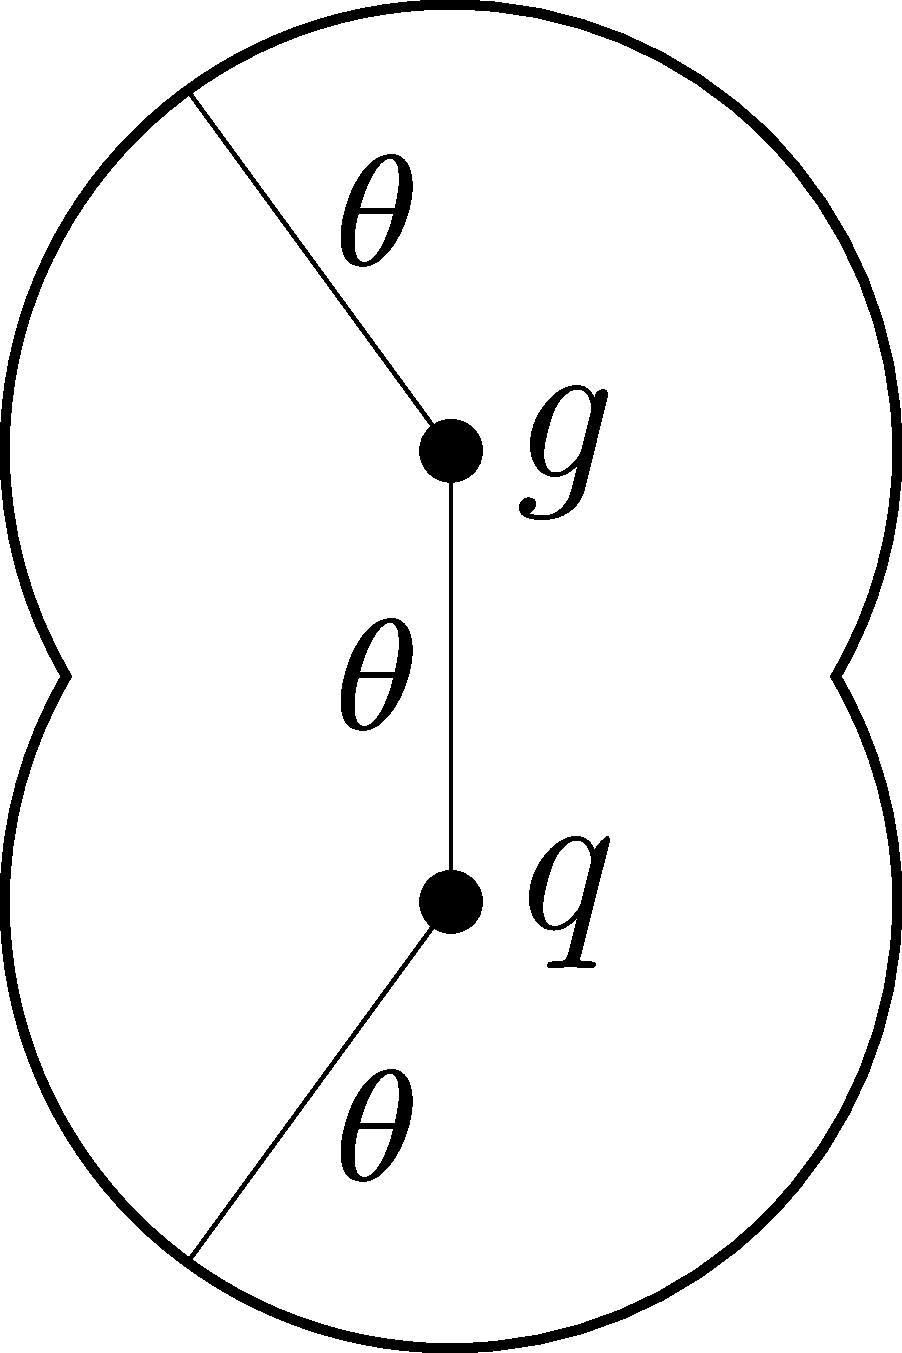
\includegraphics[width=0.2\columnwidth]{\main/factorization/figures/head_on_schematic.pdf}
		\caption{\label{fig:head-on schematic}Head-on schematic of a quark jet $q$ and a resolved gluon $g$. If the angle between the quark and the gluon is $\theta$ and the gluon (plus all lower-scale unresolved radiation) passes the groomer, then the mMDT groomer will accept all radiation within an angle $\theta$ of both the quark and the resolved gluon.}
	\end{centering}
	\end{figure}
	Unresolved soft emissions can also contribute to the jet mass if they are sufficiently close to the resolved emission or the quark. Suppose there is another emission $i$ with energy fraction $z_i$ at angle $\theta_i$ from the jet axis and angle $\theta_{iR}$ from the resolved gluon. If $\theta_i < \theta_R$ or $\theta_iR < \theta_R$, a situation displayed in Fig.~\ref{fig:head-on schematic}, then emission $i$ will pass the groomer.

	What does this mean for the hemisphere mass? Well, first notice that since $\theta_R \sim \pi/2$, most soft radiation in the hemisphere passes this cut. The effect of these extra-soft emissions, which have $z_i \ll z_R$, is to perturb the mass of the resolved emission, so that the hemisphere mass is approximately
	\begin{equation}
		\rho \sim z_R + \sum_i z_i(1 - \cos\theta_i).
	\end{equation}
	The dominant contributions come again from the wide-angle emissions with $1 - \cos\theta_i \sim 1$; these must evidently have an energy scale set by
	\begin{equation}
		\rho - z_R \sim \sum_i z_i.
	\end{equation}
	Hence, since $z_R \sim \zcut$, the unresolved extra-soft emissions must scale as
	\begin{equation}
		p_{S_R} \sim \qty(\rho - \zcut)Q(1, 1, 1).
	\end{equation}

\subsection{Groomed soft radiation}
	Radiation outside of the region displayed in Fig.~\ref{fig:head-on schematic} gets groomed away if its energy fraction is
	\begin{equation}
		z_i < \zcut.
	\end{equation}
	If $z_i > \zcut$, then we would have a second resolved emission, which we have already decided to ignore. These emissions must be at a very wide angle in order to not be within the region of mMDT acceptance. Since this \textbf{global soft} radiation is removed by the groomer, it is not sensitive to $\rho$ and contributes only to the normalization. It must scale as
	\begin{equation}
		p_{S_G} \sim \zcut Q(1, 1, 1).
	\end{equation}

\subsection{Collinear radiation}\label{sec:collinear radiation}
	Finally, we consider radiation collinear to a jet axis with angle $\theta_i \ll 1$. This radiation has $p^- \gg p^+$, which means from Eq.~\ref{eq:z light cone coordinates} that
	\begin{equation}
		z \approx \frac{p^+}{2Q}.
	\end{equation}
	Then because the particle must satisfy
	\begin{equation}
		z_i \theta_i^2 \lesssim \rho,
	\end{equation}
	we find that \cite{frye_factorization_2016}
	\begin{equation}
		\rho \sim \frac{p^+}{Q}.
	\end{equation}

	If $z \sim 1$, we know that $z \gg \zcut$, so the momentum scales independently of $\zcut$. Hence, the scaling of these \textbf{collinear} modes is \cite{frye_factorization_2016}
	\begin{equation}
		p_c \sim Q \qty(1, \rho, \rho^{1/2}).
	\end{equation}
	In a hemisphere where the resolved emission stops the mMDT groomer, this is the only collinear radiation that contributes {\color{red}\textbf{[TODO: ask Andrew: is this correct?]}}.

	If on the other hand $z \sim \zcut \ll 1$, the result is \textbf{collinear-soft} radiation with $p^- \sim z_i Q$ and $p^+ \sim \theta_i^2 z_i Q$. From \cite{frye_factorization_2016}, these momenta scale like
	\begin{equation}
		p_{cs} \sim \zcut Q \qty(1, \frac{\rho}{\zcut}, \qty(\frac{\rho}{\zcut})^{1/2})
	\end{equation}
	and depend on the single energy scale $\sqrt{\rho\,\zcut}$. This scale matters in the hemisphere which does not contain the resolved soft gluon.


\section{Factorization}
	With the power counting in hand, we are now ready to derive a factorization formula describing the hemisphere mass distribution in the limit $\rho \sim \zcut \ll 1$. First, we should note that it is most straightforward to compute the double differential cross section in the masses of the individual hemispheres, then integrate over them to get the heavy hemisphere mass \cite{chien_resummation_2010}:
	\begin{equation}\label{eq:heavy hemisphere cross section}
		\frac{d\sigma}{d\rho} = \int \frac{d^2\sigma}{d\rho_1d\rho_2}\qty[\delta(\rho - \rho_1)\Theta(\rho_1 - \rho_2) + \delta(\rho - \rho_2)\Theta(\rho_2 - \rho_1)].
	\end{equation}
	The integral simply breaks up the two cases $\rho_1 > \rho_2$ and $\rho_2 > \rho_1$ and assigns the correct value of $\rho$ in each case.

	Now, in the limit $\rho_1, \rho_2 \ll 1$, we can apply the technology of SCET to factorize the double-differential cross section into a product of hard, soft, and jet contributions \cite{frye_factorization_2016,ellis_jet_2010}. The basic form is
	\begin{equation}
		\frac{d^2\sigma}{d\rho_1 d\rho_2} = H(Q^2) \otimes S(\rho_1, \rho_2, \zcut) \otimes J(\rho_1) \otimes J(\rho_2).
	\end{equation}
	The symbol $\otimes$ represents convolution. Here, $Q^2$ is the squared center-of-mass energy of the collision. $H(Q^2)$ is hard function representing the cross section of $e^+ e^- \to q\bar{q}$ events, $S(\rho_1, \rho_2, \zcut)$ is the function representing soft contributions (which are sensitive to $\zcut$), and $J(\rho)$ is a function describing the production of jets with hemisphere mass $\rho$.

	As this factorization currently stands, several terms depend on multiple scales and must be refactorized. In the limit $\rho \sim \zcut \ll 1$ after mMDT grooming, the soft function consists of global soft emissions which contribute only to the normalization; a resolved soft, wide-angle emission generated by a fixed-order function; and soft radiation which passes the groomer due to the resolved emission. Therefore, we can write
	\begin{equation}
	\begin{aligned}
		\frac{d^2\sigma}{d\rho_1 d\rho_2} = H(Q^2) \times S_G(\zcut) \times R(\rho_1, \rho_2, \zcut) &\times S_R(\rho - \zcut) \\
			&\otimes J_c(\rho_1, \zcut) \otimes J_c(\rho_2, \zcut).
	\end{aligned}
	\end{equation}
	Here, $S_G(\zcut)$ describes the groomed soft wide-angle radiation, $R(\rho_1, \rho_2, \zcut)$ describes the resolved emission, and $S_R(\rho - \zcut)$ describes radiation which passes the groomer in the presence of the resolved emission. We have also re-written the jet functions as $J_c(\rho, \zcut)$ to make explicit their dependence on multiple scales.

	Now, as we established in Sec.~\ref{sec:collinear radiation}, radiation collinear to the jet with energy fraction of order 1 depends only on $\rho$, and radiation with energy fraction much less than 1 depends on the scale $\sqrt{\rho\,\zcut}$. However, this soft-collinear radiation only matters in the absence of a resolved gluon emission (which stops the mMDT groomer), in which case the jet function factorizes as
	\begin{equation}
		J_c(\rho, \zcut) = J(\rho) \otimes S_C(\sqrt{\rho\,\zcut})
	\end{equation}
	The result is that we must treat each hemisphere separately. Assuming, without loss of generality, that $\rho_1 > \rho_2$, the cross section then becomes
	\begin{equation}
	\boxed{
	\begin{aligned}
		\frac{d^2\sigma}{d\rho_1 d\rho_2} = 2 H(Q^2) \times S_G(\zcut) &\times R(\rho_1, \rho_2, \zcut) \times S_R(\rho - \zcut) \\
			&\otimes J(\rho_1) \otimes \qty[J(\rho) \otimes S_C(\sqrt{\rho\,\zcut})].
	\end{aligned}
	}
	\end{equation}
	This is our final factorization formula, with the heavy hemisphere mass then given by Eq.~\ref{eq:heavy hemisphere cross section}.

\ifstandalone
\bibliographystyle{../bsts/JHEP} 
\bibliography{../jet_substructure}
\fi
\end{document}
